\documentclass[reprint,amsmath,amssymb,aps, prl]{revtex4-2}
\usepackage{graphicx}% Include figure files
\usepackage{dcolumn}% Align table columns on decimal point
\usepackage{bm}% bold math
\usepackage{amsmath}
\usepackage{natbib}
\usepackage{chngcntr}

\bibliographystyle{apsrev}
\title{Bibliography management: \texttt{natbib} package}
\setcounter{tocdepth}{5}
\setcounter{secnumdepth}{5}

\begin{document}

\preprint{APS/123-QED}

\title{Manuscript Title:\\with Forced Linebreak}% Force line breaks with \\


\author{Alon Shaaltiel}
\author{Oren Kereth}
\affiliation{Raymond and Beverly Sackler School of Physics and Astronomy, Faculty of Exact Sciences, Tel Aviv University, Tel Aviv 69978, Israel}



\date{\today}% It is always \today, today,
             %  but any date may be explicitly specified

\begin{abstract}
An article usually includes an abstract, a concise summary of the work
covered at length in the main body of the article. 
\begin{description}
\item[Usage]
Secondary publications and information retrieval purposes.
\item[Structure]
You may use the \texttt{description} environment to structure your abstract;
use the optional argument of the \verb+\item+ command to give the category of each item. 
\end{description}
\end{abstract}

%\keywords{Suggested keywords}%Use showkeys class option if keyword
                              %display desired
\maketitle
\renewcommand*{\thesection}{\arabic{section}}
\renewcommand*{\thesubsection}{\arabic{section}.\arabic{subsection}}
\renewcommand{\thefigure}{\arabic{section}.\arabic{figure}}

\section{Introduction}
In this experiment the Fourier Transform Infra Red spectrometer (FTIR) will be used extensively to extract the IR spectra of various materials and compounds. Let us start with a short historical review. In 1800 IR was recognized as a distinct region of the energy spectrum by Sir William Herschel, however the study of IR light with various materials started about 100 years later. In 1903, William W.Coblentz measured the IR spectra of hundreds of inorganic and organic compounds. As a result of increasing interest in the field, the first prototypes of IR spectroscopy were built in the 1930s.  In 1949 the astrophysicist Peter Fellgett used an interferometer to measure light from celestial bodies and produced the first Fourier transform infrared spectrum, however this method was still limited and took many hours to compute. In the late 1960s commercial FTIR spectrometers appeared because microcomputers were able to do the Fourier transform, however they were large and expensive. Over time, technology reduced the costs, increased availability and enhanced the capabilities of FTIR spectroscopy systems\cite{spechistory}


\subsection{Thin Film Interference}
Upon contact with a beam of light, the internal reflections in a thin sample of material with a sufficiently low refractive index are not negligible.
\begin{figure}[h]
    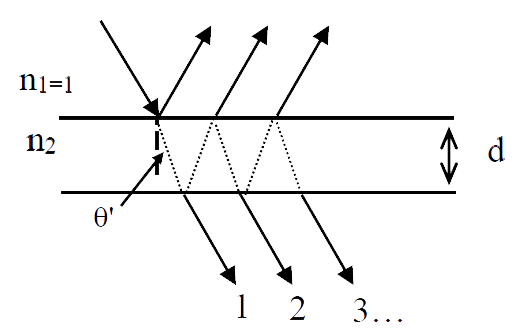
\includegraphics[width=\linewidth]{Images/Thin film.png}
    \caption{Reflected and transmitted light waves from a thin film}
    \label{fig:ThinFilm}
\end{figure}

This experiment concerns only the transmitted beams; The reflected beams are quite similar. The phase between two consecutive transmitted beams and relative intensity are
\begin{equation} \label{eq:ThinPhaseAmp}
\Delta\varphi=2n_{2}dcos(\theta);\frac{I_{n+1}}{I_{n}}=r^{2}
\end{equation}
where r is the reflection coefficient of the material and is smaller than 1, d is the sample's thickness, $\theta$ is the beam's angle inside the sample, $n_{2}$ is the sample's refractive index and $I_{n}$ is the n-th transmitted beam's intensity. Constructive interference occurs if $\Delta\varphi=\frac{m}{k}$ and if $\Delta\varphi=\frac{m+\frac{1}{2}}{k}$, destructive interference occurs. The difference in k, the wavenumber, between two constructive peaks is 
\begin{equation} \label{eq:ThinDiffWavenum}
\Delta k=\frac{1}{2n_{2}dcos(\theta)}
\end{equation} 
The transmitted intensity $I_{tot}=\sum I_{i}$ is proportional to $sin(\frac{1}{\Delta k}k)+{\it const}$.

% By measuring both $\Delta k$ using a Fourier transform of the intensity or a sine fit, and the thickness of the sample in the lab, the material's refractive index can be extracted 
% \begin{equation} \label{eq:ThinRefractIndex}
% n_2=\frac{1}{2\Delta kdcos(\theta)}
% \end{equation}

\subsection{The Beer-Lambert Law}
The Beer-Lambert Law describes how a monochromatic beam of light is absorbed in relation to substance concentration. The dependency is given by
\begin{equation} \label{eq:BeerLambert}
ln\left(\frac{P(v)}{P_{0}(v)}\right)=A=-av_{\alpha\alpha'}Cx
\end{equation}
where $P(v)$ is the light's intensity through the sample, $P_{0}(v)$ is the intensity with no sample, $A$ is the absorbance, $a$ is the molar attenuation coefficient, $\alpha$ and $\alpha'$ are quantum numbers, $C$ is the concentration, and $x$ is the optical path length of the beam. All else being equal, the absorbance and concentration are proportional to one another.

\subsection{CO Molecule IR Spectrum}
The model used to describe this molecule and other diatomic molecules pictures a molecule in which the individual atoms, held together by chemical bonds, are in vibratory motion along these bonds, while the molecule as a whole is rotating \cite{alpert}. The energy states of this system correspond to a Hamiltonian with a potential 
\begin{equation} \label{eq:CO_Potential}
V(\boldsymbol{r})=\frac{1}{2}k(r-r_0)^2
\end{equation}
and can be expressed as a combination of rotational and vibrational energies
\begin{equation} \label{eq:CO_RotVibEnrg}
E=E_{Rot}+E_{Vib}= hcw_{e}(\nu +\frac{1}{2}) + \frac{\hbar  ^2}{2I}J(J+1)
\end{equation}
where $h$ is Planck's constant, $c$ is the speed of light, $w_{e}$ is the wave number corresponding to the frequency of vibrations, $\nu$ is a quantum number corresponding to the vibrations,  $I$ is the molecule's moment of inertia and $J$ is a quantum number corresponding to the angular momentum of the particle \cite{griffithsQM}. However, the potential is not truly harmonic, as effects such as the centrifugal force, Coriolis and Fermi \cite{alpert} require the use of perturbation theory \cite{samurai}. Using the perturbation theory, the energy states are now
\begin{equation} \label{eq:CO_PeturbRotVibEnrg}
\begin{split}
T & =T_{Vib}+T_{Rot}=\\
& w_{e}(\nu +\frac{1}{2}) -w_{e}x_{e}(\nu +\frac{1}{2})^2+ \\
& B_{v}J(J+1)-D_{v}J^2(J+1)^2 
\end{split}
\end{equation}
where $x_{e}$, $B_{v}$ and $D_{v}$ are constants which take into account small perturbations and $T$ is the energy states in wave number units ($T=\frac{E}{hc}$). At room temperature only the $\nu=0$ state is occupied while the $J$ states are all occupied. Therefore, using selection rules \cite{griffithsQM} only the transitions $\nu$ $\rightarrow $ $\nu'$  where $\nu ' =1,2,3$  and $J$ $\rightarrow $ $J'$ where $J'=J+1,J-1$   are of interest. Using equation (\textbf{need to add reference for the right equation)} the allowed spectral lines are derived to be
\begin{equation} \label{eq:CO_DiffPeturbEnrg}
\begin{split}
& \Delta T =T(\nu ',J')-T(0,J)=\\
& w_{e}\nu' -w_{e}x_{e}(\nu'^{2})+(2B_{e}-\alpha(\nu'+1))m-\\
& \alpha\nu'm^2-4D_{v}m^{3}
\end{split}
\end{equation}
where $\Delta T$ is the allowed spectral line, $B_{e},\alpha $ are constants related to $B_{v}$  which are the result of further corrections due to perturbation theory and $m$ is either $J+1$ or $-(J-1)$  depending on the transition. In this experiment the transitions to $\nu'=1$ and $\nu' =2$ will be of interest, for which $\Delta T=2141\frac{1}{cm}$ and $\Delta T = 4255 \frac{1}{cm}$ respectively. (maybe put a reference, maybe it's in STUART)


\section{Experimental System and Measurements}
There are two main measuring instruments in this experiment- FTIR and ATR. Both use Michelson interferometers and perform a Fourier transform.

\subsection{Michelson Interferometers}
A Michelson interferometer consists of two perpendicularly plane mirrors, one of which can travel in a direction perpendicular to the plane. A semi reflecting film, the beamsplitter, bisects the planes of these two mirrors. The beamsplitter splits the beam into two, one beam transmitted through the beamsplitter and the other reflected from it. Both beams then get reflected from the mirrors, returning to the beamsplitter where they recombine and interfere \cite{stuart} (see Figure 2). 
\begin{figure}[h]
    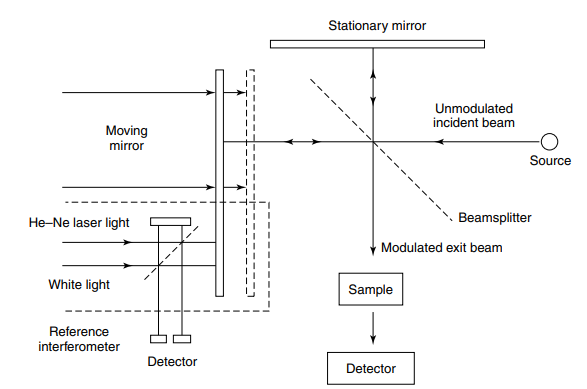
\includegraphics[width=7cm]{Images/INTERFEROMETER.png}
    \caption{Schematic of a Michelson interferometer \cite{stuart}.}
    \label{fig:Interferometer}
    \centering
\end{figure}
The beam which emerges from the interferometer at 90 degrees to the input beam is called the transmitted beam and is the beam detected by the detector. The moving mirror produces an optical path difference between the two beams split by the beamsplitter. Plotting the signal produced as a function of the change of pathlength between the two beams will yield an interferogram. By performing a Fourier transform on the interferogram the spectral distribution of the beam (i.e. the amplitude of each wave number the light is consisted of) can be found.
\subsection{FTIR}
FTIR stands for Fourier transform infrared. IR radiation is passed through a sample.
Some of the infrared radiation is absorbed by the sample and some of it is
passed through (transmitted). The resulting spectrum represents the molecular
absorption and transmission \cite{FTIRmanual}. FTIR (see Figure 3) utilises Michelson interferometers, the interferogram and a Fourier transform to perform the analysis of the spectrum. 
\begin{figure}[h]
    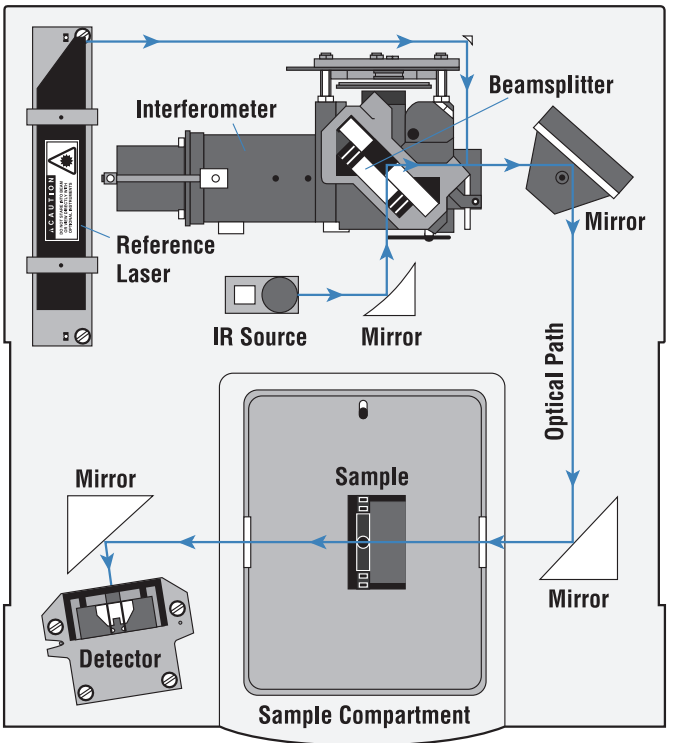
\includegraphics[width=7cm]{Images/FTIR LAYOUT.png}
    \caption{Layout of the FTIR spectrometer \cite{FTIRmanual}.}
    \label{fig:FTIR}
    \centering
\end{figure}

The main components of the FTIR spectrometer are the source, a black-body source from which the IR radiation is emitted. The radiation then passes through an interferometer, where the 'spacial encoding' takes place \cite{FTIRmanual}. A He-Ne laser is used as a reference for calibration of the moving mirror's position \cite{stuart}. After going through the interferometer, an interferogram is created. The interferogram then passes through the sample, where specific wave numbers are absorbed according to the sample's characteristics and the rest are transmitted into the detector where the interferogram signal is measured. The data reaches the computer, which performs a Fourier transform yielding the infrared spectrum consisting of absorption lines corresponding to the sample. 

\subsection{ATR}
ATR, which stands for Attenuated Total Reflection, measures the absorbance of a liquid or solid using IR spectroscopy. A crystal with a sufficiently high refractive index to achieve total internal reflection is surrounded by the material whose absorbance is measured. 
\begin{figure}[h]
    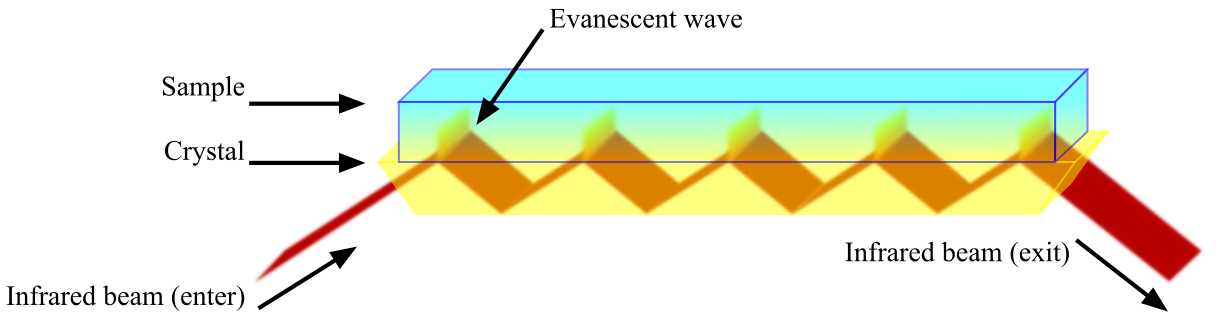
\includegraphics[width=7cm]{Images/ATR.png}
    \caption{Layout of an ATR compartment \cite{wiki:ATR}}
    \label{fig:ATR}
    \centering
\end{figure}
An interferogram is projected into the crystal and evanescent waves, resulting from the total internal reflection, propagate through the sample. In a vacuum, the energy evanescent waves carry is wholly returned. However, when a sample is inserted, wavelengths corresponding with the sample's normal modes are absorbed. As other wavelengths are not affected, the loss in intensity across the interferogram is very small when compared with a projection through the sample. As described in the previous paragraph, the interferogram is detected and disassembled into the sample's infrared spectrum.

\subsection{Transmission Through Thin Films of Polyester}
In this part of the experiment the refractive index of a thin sample of Polyester is extracted. Thin Polyester samples with varying widths are placed in the sample area perpendicular to the beam's direction. An interferogram is projected through each sample. The resulting IR spectrum will include both the absorbance spectrum of the Polyester and the sine wave of thin film interference. To extract the frequency of interference an area of low absorbance in the spectrum is sought out, and a sine wave is fitted.  Using equation \ref{eq:ThinDiffWavenum}, the extracted sine frequency, the measured width and under the assumption that $\theta =\frac{\pi}{2}$ a fit of the form
\begin{equation}
    \label{eq:ThinLinFit}
    d=a_{0}+a_{1}f_{fit}
\end{equation}
was made. Where $d$ is the sample width, $f_{fit}$ is the frequency of the fitted sine with a theoretical value of $\frac{1}{\Delta k}$, $a_{1}$ is the slope with a theoretical value of $2n_{2}$ and $a_{0}$ is the constant with a theoretical value of 0. Using the relation between the fitted frequency and width, the widths of three samples were found.

\subsection{Calibration Using Ethanol} 
In this part of the experiment the relationship between the concentration of a dissolved substance inside a solution to its total absorbance amplitude, which is assumed to be linear according to equation \ref{eq:BeerLambert} was calibrated. The calibration was done using mixtures of water and ethanol  with varying known concentrations. The mixture was put into a tank inside an ATR. Starting from a concentration of $96\%$ , the ethanol was diluted by adding more water into the mixture, thus changing the concentration of the ethanol according to 
\begin{equation} \label{eq:EthanolConcentrVolume}
C_{i}V_{i} = C_{f}V_{f}
\end{equation}
where $C_{i}$,$V_{i}$, $C_{f}$,$V_{f}$ are the initial and final concentration of ethanol and volume of the mixture respectively. 
For each concentration, $F$ , the total absorbance of ethanol in the range $1000-1120 \frac{1}{cm}$ was calculated and a calibration graph of the form 
\begin{equation} \label{eq:EthanolLinFit}
    C=a_{0}+a_{1}F 
\end{equation} 
was made. Where C is the concentration of ethanol in the mixture. Using the calibration, the concentration of different solutions was found. 

\subsection{CO2 and IR Spectrum of CO}
Using a pump, exhaled and outside air were each inserted into a chamber in the FTIR. For each of the two types of air the total absorbance in the IR spectrum in the range $2270-2400\frac{1}{cm}$ were calculated. In this region there are two absorption peaks both corresponding to the concentration of CO2 in the air. The ratio between the total absorbance of the exhaled air to the outside air in that region, denoted by $S$ is therefore equal to the corresponding ratio between CO2 concentrations in each of them. $S$ will then be compared to ratios previously measured. 
Afterwards, by pumping CO into to the same chamber in the FTIR and its IR spectrum was measured.  According to equation 8 ,  the spectrum contains absorption peaks that represent a transition in the angular momentum of the molecule, $J$  to either $J+1$ or $J-1$ (see Figure 5)  
\begin{figure}[h]
    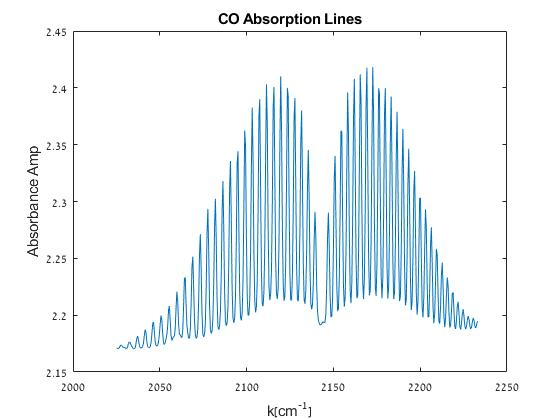
\includegraphics[width=7cm]{Images/COEnergystates.jpg}
    \caption{CO absorption lines in the region $2025-2033 \frac{1}{cm}$. Each peak represents a transition $m$ of the angular momentum and the transition from $\nu=0$ to $\nu'=1$ which is centered at 2142$\frac{1}{cm}$  as can be seen and according to subsection 1.3.}
    \label{fig:CoEnergy}
    \centering
\end{figure}
Each of the peaks, $m$ , were numbered according to its order relative to the center point at 2142$\frac{1}{cm}$ (i.e. if $m$ was the first to its left it was numbered as $-1$ and if it was the first to its right it was numbered as $1$). Afterwards, a polynomial fit of $3^{rd}$ order was made between $\Delta T$ from equation 8 and $m$
\begin{equation} \label{eq:CO_EnrgStatesFit}
    \Delta T = a_{0}+a_{1}m+a_{2}m^2+a_{3}m^3
\end{equation}
The coefficients extracted from the fit will then be used to extract the coefficients in equation 8 according to the relations 
\begin{equation}
\begin{aligned}
\alpha &=-a_{2} & D_{v}&=-\frac{a_{3}}{4} & w_{e}&=2a_{0}-\frac{4255}{2} \\
B_{e}&=\frac{a_{1}-2a_{2}}{2} &  x_{e}&=\frac{a_{0}-\frac{4255}{2}}{2a_{0}-\frac{4255}{2}}
\end{aligned}
\label{eq:COFITcoefficients}
\centering
\end{equation}
where in order to find $w_{e}$ and $x_{e}$ the spectral line of the transition $\nu =0 \rightarrow \nu'=2$ and $\Delta J =0$ was used. 

\subsection{IR Spectra of Different Cigarette Brands}
In this part of the experiment gasses in the smoke of various cigarettes are analyzed. An interferogram is projected through regular air. A pump smokes on a cigarette and fills the sample area with smoke. An interferogram is projected through the smoke and the absorbance spectrum compared to regular air is created. Various toxic gasses are identified. The gasses' concentrations are estimated using the area of the absorbance peaks.

\section{Results}
\subsection{Ethanol Concentration Calibration}
The total absorbance amplitude in the range $1000-1120 \frac{1}{cm}$ was calculated numerically for each concentration of ethanol in the mixture using the trapezoidal method\cite{numerical}. Plotting the IR spectrum of all the mixtures in that range on the same graph (see Figure 6) shows the increasing intensity of the peaks for higher and higher concentrations of ethanol. 
\begin{figure}[h]
    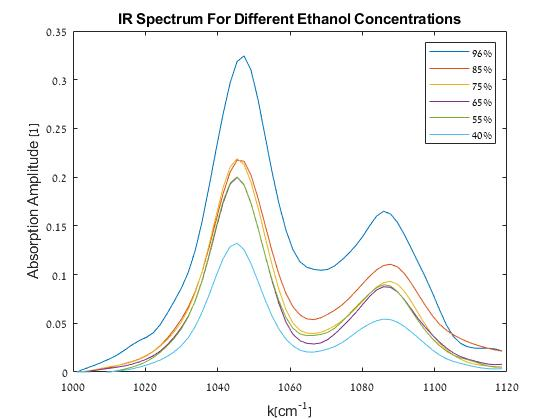
\includegraphics[width=7cm]{Images/EthanolAbsorption.jpg}
    \caption{IR spectrum of mixtures with different ethanol concentration in the range 1000-1120$\frac{1}{cm}$ }
    \label{fig:EthanolMixtures}
    \centering
\end{figure}

Fitting a linear function according to equation \ref{eq:EthanolLinFit} to the measurements of concentration and absorbance yielded the following (see Figure 7).
    \begin{figure}[h]
    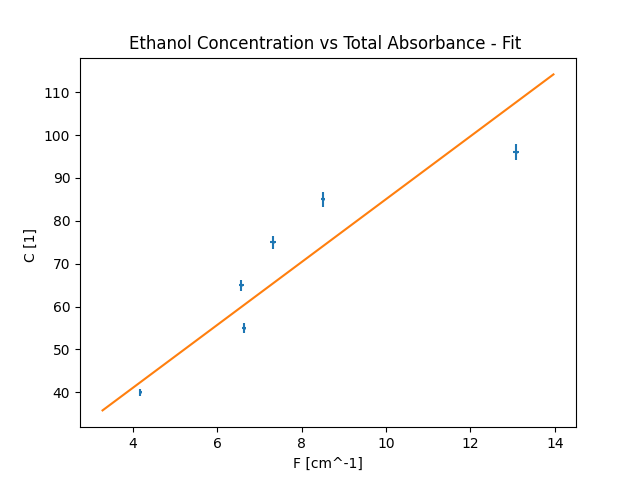
\includegraphics[width=7cm]{Images/linear_fittingethanol}
    \caption{Linear calibration graph of concentration of ethanol in the mixture to total absorbance amplitude in the range $1000-1120 \frac{1}{cm}$}
    \label{fig:EthanolCalibration}
    \centering
\end{figure}
The fit parameters extracted from the linear fit can be seen in Table 1
\begin{table}[h]
\begin{tabular}{ |p{2cm}||p{2cm}|p{2cm}|  }
 \hline
 \multicolumn{3}{|c|}{Fit Parameters of Ethanol Calibration Graph} \\ \hline
 Parameter& Value &Error (Relative Error)\\ \hline
 $a_{0}$[$1$]    &$11.7$    &$9.3$($79\%$) \\
 $a_{1}$[$cm$] &$7.3$    & $1.4$ ( $19\%$)  \\ \hline
\end{tabular}
\caption{\label{ethanol table}Fit parameters of the ethanol concentration vs absorption amplitude graph}
\end{table}
The concentration of ethanol in other mixtures was then found by numerically calculating the total absorption in the relevant range and plugging it in the linear equation using the fit parameters. Using the fit parameters from Table 1 the concentrations in a Suktinis and two unknown alcoholic beverages were found (see Table 2).

\begin{table}[h]
\begin{tabular}{ |p{2.8cm}||p{2.8cm}|p{2.8cm}|  }
 \hline
 \multicolumn{3}{|c|}{Ethanol Concentration in Different Beverages} \\
 \hline
 Beverage& Concentration(\%) &Concentration Error (Relative Error) \\ \hline
Sukinis    &$54.3$  &$8.3$ ($15\%$) \\
Unknown 1 &$40.5 $  &$5.7$  ($14\%$) \\
Unknown 2  &$72$     & $12$ ( $17\%$) \\ \hline
\end{tabular}
\caption{\label{beverages table}Ethanol concentration in different beverages}
\end{table}

\subsection{\label{subsec:level20} CO2}
Using the trapezoidal method to calculate the total absorbance of the air in the region $2270-2400\frac{1}{cm}$ which correlates to the concentration of CO2 (CITE THE WEBBOOK AGAIN!), the ratio between CO2 in exhaled air to outside air, S,  was calculated yielding 
\begin{equation}
\label{eq:CO2ratio}
S=61[1]
\end{equation}
This value would be later compared to that measured a few years ago to see the trend line.  
\subsection{\label{subsec:level21}CO}
The absorption peaks from the IR spectrum of CO were extracted and the absorption lines $\Delta T$ and their corresponding angular momentum transitions $m$ were measured relative to the center point at $\Delta T=2141 \frac{1}{cm}$ which represents $\Delta J = m = 0 $ and the vibrational transition from $\nu =0$ to $\nu' =1$ . Using that data, a $3^{rd}$ order polynomial fit was made according to equation \ref{eq:CO_EnrgStatesFit} (see Figure 8). 
\begin{figure}[h!]
    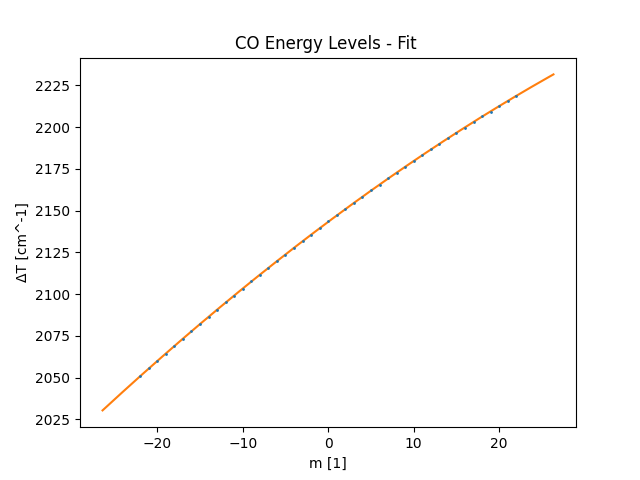
\includegraphics[width=7cm]{Images/polynomial_3_fitting.png}
    \caption{$3^{rd}$ order polynomial fit of the spectral lines of the absorption peaks $\Delta T$ as a function of the transition of the molecule's angular momentum $m$. }
    \label{fig:COPolynomialfit}
    \centering
\end{figure}
The fit parameters extracted can be seen at Table 3. 
\begin{table}[h]
    \resizebox{9cm}{!}{
    \begin{tabular}{ |p{2.8cm}||p{2.8cm}|p{2.8cm}|  }
    
     \hline
     \multicolumn{3}{|c|}{Fit Parameters of the CO absorption lines $3^{rd}$ polynomial fit} \\
     \hline
     Parameter& Value(\%) & Error (Relative Error) \\ \hline
    $a_{0}[\frac{1}{cm}]$    &$2143.293$  &$0.034$ ($0.002\%$) \\
    $a_{1}[\frac{1}{cm}]$  &$3.8220 $  &$0.0040$  ($0.11\%$) \\
    $a_{2}[\frac{1}{cm}]$  &$-0.01800$     & $1.5e-4$ ( $0.83\%$) \\ 
    $a_{3[\frac{1}{cm}]}$  &$-9.4e-6$     & $1.30e-5$ ( $140\%$) \\ \hline
    \end{tabular}
    }
    \caption{\label{COfittable}Fit parameters of the $3^{rd}$ order polynomial fit}
    \end{table}
Using these fit parameters the coefficients at equation \ref{eq:CO_DiffPeturbEnrg} were extracted via the relations stated at equation \ref{eq:COFITcoefficients} (see Table 4).
\begin{table}[h]
    \resizebox{9cm}{!}{
    \begin{tabular}{ |p{2.8cm}||p{2.8cm}|p{2.8cm}|  }
    
     \hline
     \multicolumn{3}{|c|}{Coefficients of The CO Absorption Lines Equation (equation \ref{eq:CO_DiffPeturbEnrg})} \\
     \hline
     Parameter& Value(\%) & Error (Relative Error) \\ \hline
    $w_{e}[\frac{1}{cm}]$    &$2159.086
    $  &$0.068
    $ ($0.0031\%$) \\
    $x_{e}[1]$  &$0.007315
    $  &$1.6E-05
    $  ($0.22\%$) \\
    $B_{e}[\frac{1}{cm}]$  &$1.9290
    $     & $0.0090
    $ ( $0.47\%$) \\ 
    $\alpha$ [$\frac{1}{cm}$] & $0.01800
    $ &$1.5E-04$ ($0.83\%)
    $ \\
    $D_{v}$ [$\frac{1}{cm}$] & $2.4E-06
    $ & $3.3E-06$ ($140\%$)
     \\ \hline
    \end{tabular}
    }
    \caption{\label{COcoeftable}The coefficients from equation \ref{eq:CO_DiffPeturbEnrg} of the CO absorption lines extracted using the fit parameters}
    \end{table}


\subsection{Polyester Refractive Index Calculation}
For each sample width the area with the clearest sine wave in the absorption spectrum was found and fitted to a sine wave.
\begin{figure}[h]
    \label{fig:SineFitEx}
    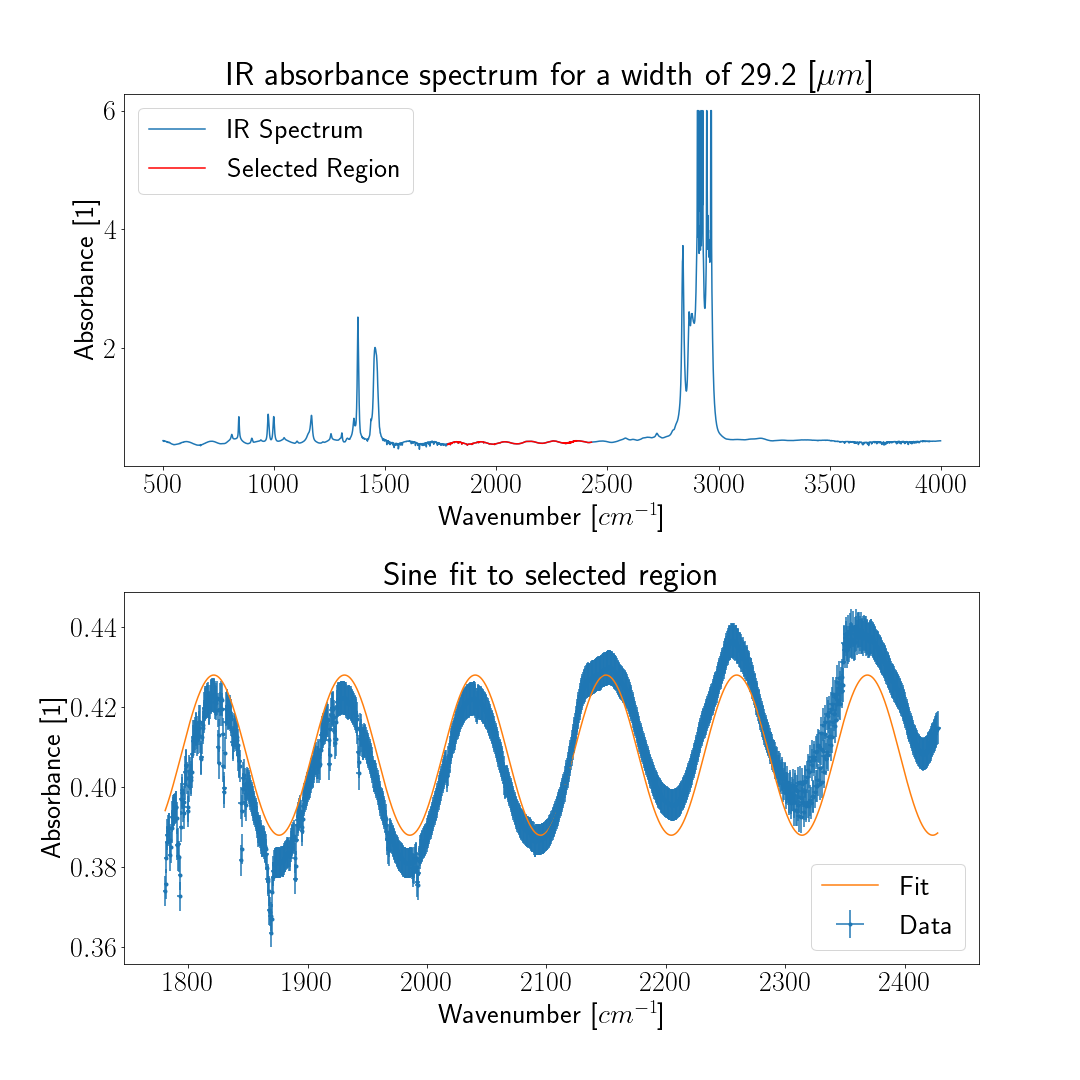
\includegraphics[width=\linewidth]{Images/29_2_Spec.png}
    \caption{IR absorbance spectrum and sine fit to the selected region for a width of $29.2\ [\mu m]$}
    \centering
\end{figure}
Fitting a linear function between the width and the frequency yielded the following (See Figure \ref{fig:ThinLinWidthFreq})
\begin{figure}[h]
    \label{fig:ThinLinWidthFreq}
    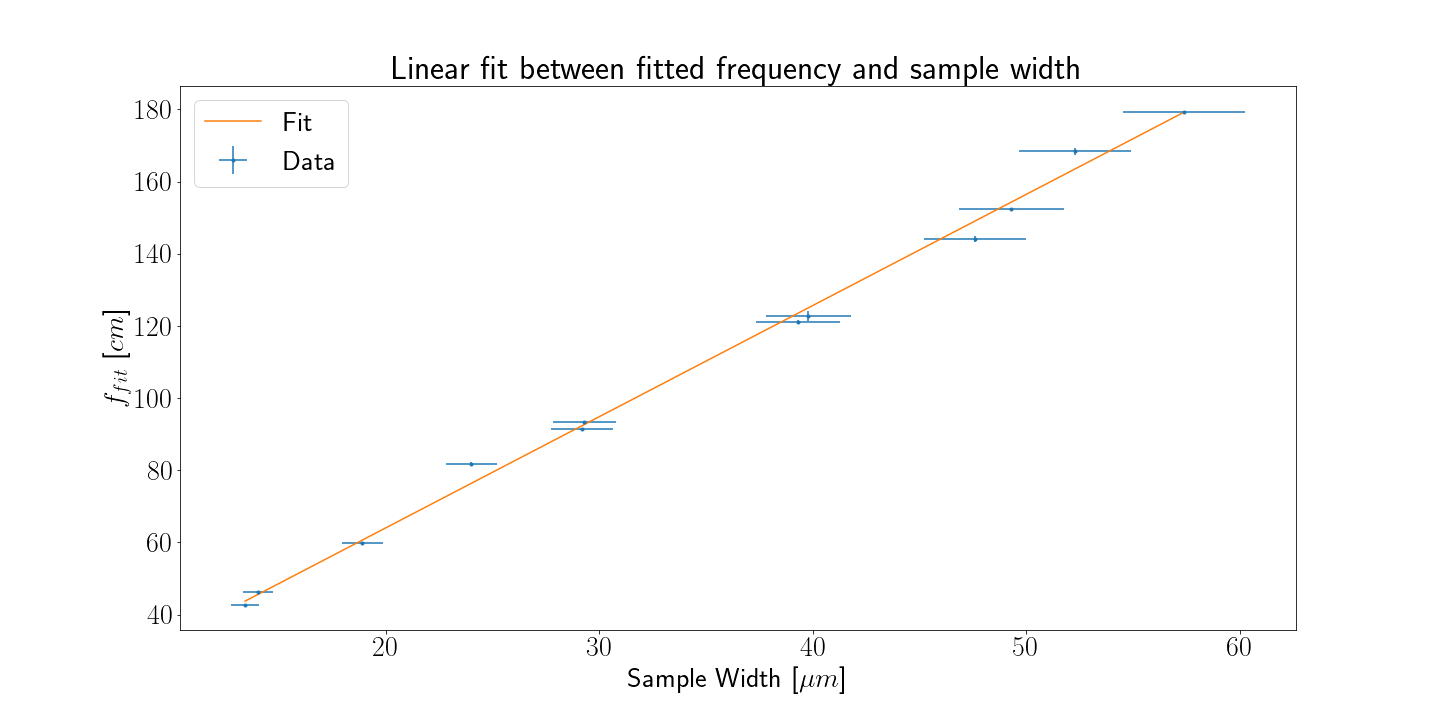
\includegraphics[width=\linewidth]{Images/__linear_fit.png}
    \caption{Linear fit between the fitted frequency, $f_{fit}$, and the sample width.}
    \centering
\end{figure}

\bibliography{Report}

\end{document}